\section{Adjoint Studies}
\renewcommand\tikzscale{1.3}


% ============================================
% ====== Frame : Adjoint State Method  =======
% ============================================

\begin{frame}{Adjoint State Method}
\scriptsize
Lagrangian functional \footcite{plessixReviewAdjointstateMethod2006} :

  \begin{equation}
    \Lag(\qcqU,\qcqLbd,\model) = \frac{1}{2}||\textcolor{blue}{d_{obs}}-\textcolor{red}{\mathcal{R}(\qcqU)}||^2 + <\DP(\qcqU)-f_p,\qcqLbd>
  \end{equation}


  \uncover<2->{
    \begin{block}{Adjoint Equation:}
  Let us choose $\qcqLbd=\contLbd$ such as $\frac{\partial \Lag}{\partial \contU} = 0$

  \begin{equation}
 \DP^*(\contLbd) + \mathcal{R}^*(\textcolor{blue}{d_{obs}}-\mathcal{R}\contU) = 0
  \end{equation}
  \end{block}
  }

  \uncover<3->{
    \begin{block}{Gradient Expression:}
  For $\DP(\contU)-f_p = 0$ :

  \begin{equation}
    \partial_{\model_i} \CF(\model) = \partial_{\model_i} \Lag(\contU,\contLbd,\model) = \partial_{\model_i} <\DP(\contU),\contLbd>
  \end{equation}
  \end{block}
  }

\end{frame}











% ============================================
% ====== Frame : Adjoint Scheme      =========
% ============================================
\begin{frame}{Adjoint Formulation}
\begin{figure}

\definecolor{color1}{RGB}{255,174,41}   %% myOrange
%\definecolor{color2}{RGB}{216,93,99}  %% myGreen
\definecolor{color3}{RGB}{100,149,237} %% myBlue
\definecolor{color2}{RGB}{223,83,74} %% myRed

\definecolor{colorOne}{RGB}{255,174,41}   %% myOrange
%\definecolor{color2}{RGB}{216,93,99}  %% myGreen
\definecolor{colorThree}{RGB}{100,149,237} %% myBlue
\definecolor{colorTwo}{RGB}{223,83,74} %% myRed


\begin{tikzpicture}[scale=\tikzscale] %% [every node/.style={scale=1}]

\node[boxOptions]
at (0,3.5){ {\textbf{\Large\fontfamily{pzc}\selectfont Continuous \\ Direct Problem}}};

\uncover<2->{
\node[boxOptions]
at (6,3.5){ {\textbf{\Large\fontfamily{pzc}\selectfont Continuous \\ Adjoint Problem}}};

\coordinate (a) at (1.4,3.5);
\coordinate (b) at (4.7,3.5);
\draw[->, >=latex, red!50!white, line width=10pt]   (a) to node[pos=0.4,above]{\small{\textbf{\textcolor{black}{Adjoint}}}} (b) ;
}

\uncover<3->{
\node[boxOptions]
at (6,0.7){\textbf{Discretization of the Continuous Adjoint Problem}};

\draw[arrowStyleinv]
(6,2.1) to[out=90,in=90]
node[sloped,anchor=south]
{}
(6,2.6);

\coordinate (b) at (6,1.2);
\coordinate (a) at (6,3.0);
\draw[->, >=latex, red!50!white, line width=10pt]   (a) to node[fill=colorThree!0,pos=0.3]{\small{\textbf{\textcolor{black}{Discretization}}}} (b) ;
}


\uncover<4->{
\node[boxOptions]
at (0,-0.5){\textbf{Discrete \\Direct Problem}};

%% \draw[arrowStyleinv]
%% (0,0.7) to[out=90,in=90]
%% node[sloped,anchor=south]
%% {\footnotesize{Discretization ~~~~~~~~~~~~~}}
%% (0,2.5);

\coordinate (b) at (0,-0.1);
\coordinate (a) at (0,3.0);
\draw[->, >=latex, blue!50!white, line width=10pt]   (a) to node[fill=colorThree!0]{\small{\textbf{\textcolor{black}{Discretization}}}} (b) ;


\node[boxOptions]
at (6,-0.5){\textbf{Adjoint of the Discrete Problem}};


%% \draw[arrowStyle]
%% (2,0) to[out=0,in=180]
%% node[sloped,anchor=south]
%% {(*)}
%% (4,0);

\coordinate (a) at (1.4,-0.5);
\coordinate (b) at (4.7,-0.5);
\draw[->, >=latex, blue!50!white, line width=10pt]   (a) to node[pos=0.4,below]{\small{\textbf{\textcolor{black}{Adjoint}}}} (b) ;
}

\uncover<5->{
\draw[color=red,line width=2] (4.5,1.4)
rectangle (7.5,-1.0);
}
\end{tikzpicture}
\end{figure}
\end{frame}








% ============================================
% ====== Frame : Adjoint then discretize 1 ===
% ============================================

\begin{frame}{OtD : Optimize then Discretized Strategy \footcite{tarantolaInversionSeismicReflection1984}}
\scriptsize
  \begin{equation}
    \CF(\contP)=\frac{1}{2}||\textcolor{blue}{d_{obs}} - R\contP||^2
    \end{equation}

  \noindent
  \begin{multicols}{2}
    \noindent
      \begin{empheq}[left=\empheqlbrace]{align}
    & \frac{1}{\density \velocity^2}\frac{\partial \contP}{\partial t}+\nabla \cdot \contV=f_p \text{~~ on $\boldsymbol{\Omega}$}\\
    & \density\frac{\partial \contV}{\partial t}+\nabla\contP=0  \text{~~ on $\boldsymbol{\Omega}$}\\
    & \contP=0 \text{~~ on $\textcolor{\myred}{\boldsymbol{\Gamma_1}}$} \\
    & \contP-\velocity \density \contV \cdot \normal=0 \text{~~ on $\textcolor{\myblue}{\boldsymbol{\Gamma_2}}$}\\
    & \contP(0) = 0 \text{, ~~~} \contV(0) = 0
      \end{empheq}
\vfill
    \columnbreak
    \noindent
    \uncover<2->{
      \vspace{-0.5cm}
      \begin{empheq}[left=\empheqlbrace]{align}
    & \hspace{0.2cm} \frac{1}{\density \velocity^2}\frac{\partial \Lbdun}{\partial t}+\nabla \cdot \Lbdeux=R^*(R\contP - \textcolor{blue}{d_{obs}})(\Tfinal -t)\\
    &  \hspace{0.2cm} \density\frac{\partial \Lbdeux}{\partial t}+\nabla\Lbdun=0  \text{~~ on $\boldsymbol{\Omega}$}\\
    &  \hspace{0.2cm} \Lbdun=0 \text{~~ on $\textcolor{\myred}{\boldsymbol{\Gamma_1}}$} \\
    &  \hspace{0.2cm}  \Lbdun - \velocity \density \Lbdeux \cdot \normal=0 \text{~~ on $\textcolor{\myblue}{\boldsymbol{\Gamma_2}}$}\\
    &  \hspace{0.2cm} \Lbdun(T) = 0 \text{, ~~~} \Lbdeux(T) = 0
      \end{empheq}
      \vfill
      }
  \end{multicols}
  \vspace{-0.5cm}
  \begin{equation}
    t\in[0,T] \uncover<2->{\text{~~~~~~~~~~~~~~~~~~~~~~~~~~} t\in[T,0]}
  \end{equation}

\end{frame}



% ============================================
% ====== Frame : Adjoint then discretize 1 ===
% ============================================

\begin{frame}[noframenumbering]{OtD : Optimize then Discretized Strategy}
\scriptsize
  \begin{equation}
    \CF(\contP)=\frac{1}{2}||\textcolor{blue}{d_{obs}} - R\contP||^2
    \end{equation}

  \noindent
  \begin{multicols}{2}
    \noindent
      \begin{empheq}[left=\empheqlbrace]{align}
    & \frac{1}{\density \velocity^2}\frac{\partial \contP}{\partial t}+\nabla \cdot \contV=f_p \text{~~ on $\boldsymbol{\Omega}$}\\
    & \density\frac{\partial \contV}{\partial t}+\nabla\contP=0  \text{~~ on $\boldsymbol{\Omega}$}\\
    & \contP=0 \text{~~ on $\textcolor{\myred}{\boldsymbol{\Gamma_1}}$} \\
    & \contP-\velocity \density \contV \cdot \normal=0 \text{~~ on $\textcolor{\myblue}{\boldsymbol{\Gamma_2}}$}\\
    & \contP(0) = 0 \text{, ~~~} \contV(0) = 0
      \end{empheq}
\vfill
    \columnbreak
    \noindent
    \uncover<1->{
            \vspace{-0.5cm}
      \begin{empheq}[left=\empheqlbrace]{align}
    & \hspace{0.2cm} \frac{1}{\density \velocity^2}\frac{\partial \Lbdun}{\partial t}+\nabla \cdot \Lbdeux=R^*(R\contP - \textcolor{blue}{d_{obs}})(\Tfinal -t)\\
    &  \hspace{0.2cm} \density\frac{\partial \Lbdeux}{\partial t}+\nabla\Lbdun=0  \text{~~ on $\boldsymbol{\Omega}$}\\
    &  \hspace{0.2cm} \Lbdun=0 \text{~~ on $\textcolor{\myred}{\boldsymbol{\Gamma_1}}$} \\
    &  \hspace{0.2cm}  \Lbdun - \velocity \density \Lbdeux \cdot \normal=0 \text{~~ on $\textcolor{\myblue}{\boldsymbol{\Gamma_2}}$}\\
    &  \hspace{0.2cm} \Lbdun(T) = 0 \text{, ~~~} \Lbdeux(T) = 0
      \end{empheq}
      \vfill
      }
  \end{multicols}
  \vspace{-0.5cm}
  \begin{equation}
    t\in[0,T] \uncover<1->{\text{~~~~~~~~~~~~~~~~~~~~~~~~~~} t\in[T,0]}
  \end{equation}

  \uncover<1->{
\begin{block}{NB:}
  Having self-adjoint continuous problem enables to use the same discretization routines to simulate the forward and the adjoint state.
\end{block}
}
\end{frame}




\subsection{Discretize then Adjoint}

% ============================================
% ====== Frame : Discretize then Adjoint 1 ===
% ============================================
\begin{frame}{DtO : Discretize then Optimize Strategy}{Example With RK2}

  For any time-schemes we get :
  \begin{equation}
    \textcolor{\myblue}{\boldsymbol{L}}\discreteU=\textcolor{\myblue}{\boldsymbol{E}}\discreteF
  \end{equation}

  \uncover<2->{
  \small
      For instance wuth RK2 time-scheme we get:
    \begin{equation}
      \discreteU^{n+1}=B\discreteU^n+\textcolor{\myblue}{\boldsymbol{C_0}}\discreteF^n+\textcolor{\myblue}{\boldsymbol{C_{\frac{1}{2}}}}\discreteF^{n+\frac{1}{2}}
    \end{equation}
    }


  \uncover<3->{
\begin{equation}
  \textcolor{\myblue}{\boldsymbol{L}}\discreteU=\textcolor{\myblue}{\boldsymbol{E}}\discreteF=\discreteG
\end{equation}
\begin{equation}
  \begin{pmatrix}
    I & & & & \\
    -B&I & & & \\
    & -B&I  & & \\
    & & \ddots & \ddots   & \\
    & &  & -B &I \\
    %% \vdots & \ddots & \vdots \\
    %% 0      & \cdots & 1
  \end{pmatrix}
    \begin{pmatrix}
    \discreteU^0 \\
    \discreteU^1 \\
    \discreteU^2 \\
    \vdots \\
    \discreteU^n \\
  \end{pmatrix}=
  \begin{pmatrix}
    \discreteG^0 \\
    \discreteG^1 \\
    \discreteG^2 \\
    \vdots \\
    \discreteG^n \\
  \end{pmatrix}
\end{equation}
}
\end{frame}



% ============================================
% ====== Frame : Discretize then Adjoint 2 ===
% ============================================
\begin{frame}[noframenumbering]{DtO : Discretize then Optimize Strategy}

   For any time-schemes we get:
    \begin{equation}
      \textcolor{\myblue}{\boldsymbol{L}}\discreteU=\textcolor{\myblue}{\boldsymbol{E}}\discreteF \uncover<1->{=\discreteG}
    \end{equation}

    We are looking for a Discrete Adjoint state satisfying :
    \begin{equation}
      \textcolor{\myblue}{\boldsymbol{L^*}}\discreteLbd=-R^*(\textcolor{blue}{d_{obs}}-R\discreteU) \uncover<1->{=\discreteD}
    \end{equation}

    \uncover<2->{
    \begin{block}{Adjoint test}
    With the adjoint operator $\textcolor{\myblue}{\boldsymbol{L^*}}$ satisfying :
      \begin{equation}
    <\textcolor{\myblue}{\boldsymbol{L}}\discreteU,\discreteLbd>=<\discreteU,\textcolor{\myblue}{\boldsymbol{L^*}}\discreteLbd>
      \end{equation}
        \begin{equation}
        <\discreteG,\discreteLbd>=<\discreteU,\discreteD> \text{~~~(Adjoint Test)}
      \end{equation}


      \begin{center}
        Adjoint test succeeds $\Longleftrightarrow$  operator $\textcolor{\myblue}{\boldsymbol{L^*}}$  well established
      \end{center}
    \end{block}
    }

\end{frame}



\begin{frame}{Discretize then Optimize}

  $\textcolor{\myblue}{\boldsymbol{L^*}}$ is challenging to develop:

  \begin{itemize}
  \item<2-> Requires the adjoint operator of the fluxes \footcite{wilcoxDiscretelyExactDerivatives2013} (Reverse all the communications).
  \item<3-> Requires the development of the adjoint operator for all propagator.
  \item<4-> Architectures of the program divided into several libraries.
    \begin{itemize}
    \item<5-> Requires the development of the adjoint in each inner functions.
    \item<6-> Prevents the use of automatic differentiation tools \footcite{griewank2008evaluating}.
    \end{itemize}
  \end{itemize}

\end{frame}







% ================================================
% ====== Frame : Adjoint Strategies Comparison ===
% ================================================

\begin{frame}{Adjoint Strategies Comparison}
  \begin{columns}
    \begin{column}[t]{0.5\textwidth}
      \textbf{\textcolor{red}{Optimize Then Discretize}}
      \vspace{0.5cm}
%      \dotfill % to show column margins
      \begin{itemize}
      \item[\textcolor{\mygreen}{\textbf{+}}] Physical approach
      \item[\textcolor{\mygreen}{\textbf{+}}] Same discrete operators for Forward and Backward
      \item[\textbf{- -}] Approximate gradient \footnotemark
      \end{itemize}
      %      \dotfill
      \vspace{0.5cm}
    \end{column}\vrule \hfill
    \begin{column}[t]{0.5\textwidth}
      \uncover<2->{
      \textbf{\textcolor{blue}{Discretize then Optimize}}
      \vspace{0.5cm}
%            \dotfill
      \begin{itemize}
      \item[\textcolor{\mygreen}{\textbf{+}}] Numerical approach
      \item[\textcolor{\mygreen}{\textbf{+}}] Has an Adjoint Test
      \item[\textcolor{\mygreen}{\textbf{+}}] Exact Gradient
      \item[\textbf{-}] Not that obvious to develop
      \item[\textcolor{black}{\textbullet}] Possible inconsistency of the adjoint scheme \footnotemark
      \end{itemize}
      }
    \end{column}
  \end{columns}
  \addtocounter{footnote}{-1}
  \footcitetext{gunzburger2002perspectives}
  \addtocounter{footnote}{+1}
  \footcitetext{sei1995note}
\end{frame}


% ================================================
% ====== Frame : 1D comparison ===================
% ================================================



\subsection{1D FWI problem}
\begin{frame}{1D FWI problem}

\begin{figure}[H]
  \centering
   \begin{tikzpicture}[scale=1.5]
      \draw[color=black,line width=2.1](0.0,0.0) -- (6.5,0);
      %\draw[color=blue, line width=10] (0,-0.02) node {$\bullet$} ;
      %\draw[color=blue, line width=10] (5,-0.02) node {$\bullet$} ;
     % \draw node[color=blue,fill,circle,minimum size=0.01](1,1) {};
      \node[anchor=south east, color=black]
      at (0,0) {};
      %\node[anchor=south west, color=black]
      %at (4.0,0.2) {\Large $\velocity$ ?};

      \pgfmathsetmacro{\x}{0.0}
      \draw[color=black,line width=2.1](\x,0.1) -- (\x,-0.1);

      \pgfmathsetmacro{\x}{6.5}
      \draw[color=black,line width=2.1](\x,0.1) -- (\x,-0.1);

      \pgfmathsetmacro{\x}{0.5}
      \draw[color=black,line width=1.5](\x,0.1) -- (\x,-0.1);
      \draw[color=black,line width=1.5](\x,0.1) -- (\x,-0.1);



      \pgfmathsetmacro{\x}{1.0}
      \draw[color=black,line width=1.5](\x,0.1) -- (\x,-0.1);
      \pgfmathsetmacro{\x}{1.5}

      \draw[color=black,line width=1.5](\x,0.1) -- (\x,-0.1);
      \pgfmathsetmacro{\x}{2.0}
      \draw[color=black,line width=1.5](\x,0.1) -- (\x,-0.1);
      \pgfmathsetmacro{\x}{2.5}
      \draw[color=black,line width=1.5](\x,0.1) -- (\x,-0.1);
      \pgfmathsetmacro{\x}{3.0}
      \draw[color=black,line width=1.5](\x,0.1) -- (\x,-0.1);
      \pgfmathsetmacro{\x}{3.5}
      \draw[color=black,line width=1.5](\x,0.1) -- (\x,-0.1);
      \pgfmathsetmacro{\x}{4.0}
      \draw[color=black,line width=1.5](\x,0.1) -- (\x,-0.1);
      \pgfmathsetmacro{\x}{4.5}
      \draw[color=black,line width=1.5](\x,0.1) -- (\x,-0.1);
            \pgfmathsetmacro{\x}{5.0}
      \draw[color=black,line width=1.5](\x,0.1) -- (\x,-0.1);

            \pgfmathsetmacro{\x}{5.5}
      \draw[color=black,line width=1.5](\x,0.1) -- (\x,-0.1);


            \pgfmathsetmacro{\x}{6.0}
      \draw[color=black,line width=1.5](\x,0.1) -- (\x,-0.1);

      \pgfmathsetmacro{\x}{1.8}
      \pgfmathsetmacro{\dx}{0.2}
      \pgfmathsetmacro{\y}{-0.2}
      \pgfmathsetmacro{\dy}{-0.4}
      \node (A) at (\x,\y) {}; % B = 5
      \node (B) at (\x+\dx,\y+\dy) {}; % AC = 3
      \node (C) at (\x-\dx,\y+\dy) {}; % BC = 4
      \node (receiver) at (\x,\y+\dy-0.1) {Receiver}; % BC = 4
     % \draw (A) -- (B) -- (C) -- (A);
      \begin{scope}%[on background layer]
        \fill [blue] (A.center) -- (B.center) -- (C.center) -- cycle;
      \end{scope}

            \pgfmathsetmacro{\x}{0.6}
      \pgfmathsetmacro{\dx}{0.2}
      \pgfmathsetmacro{\y}{-0.2}
      \pgfmathsetmacro{\dy}{-0.4}
      \node (A) at (\x,\y) {}; % B = 5
      \node (B) at (\x+\dx,\y+\dy) {}; % AC = 3
      \node (C) at (\x-\dx,\y+\dy) {}; % BC = 4
      \node (source) at (\x,\y+\dy-0.1) {Source}; % BC = 4
      %\draw [red] (A) -- (B) -- (C) -- (A);
      \begin{scope}%[on background layer]
        \fill [red] (A.center) -- (B.center) -- (C.center) -- cycle;
      \end{scope}
\end{tikzpicture}

  \caption*{1D domain $\Domain$.}
  \label{1D_domain}
\end{figure}


\uncover<2->{
      \setlength{\plotwidth} {3.5cm}
      \setlength{\plotheight}{2.8cm}
      \pgfplotsset{every tick label/.append style={font=\tiny}}
      \begin{figure}[H]
      \begin{subfigure}{0.45\textwidth}
        \centering
          \begin{tikzpicture}
      \begin{axis}[%
          width=\plotwidth, height=\plotheight,,
          at={(0,0)},scale only axis,separate axis lines,xminorticks=true,
          xlabel={\scriptsize{$x$}},
          ylabel={\scriptsize{Wavespeed (m.s$^{-1}$)}},
          %ylabel={$\velocity$},
          %%   ymode=log,
          yminorticks=true,
          %xmin=0.,xmax=100.,
          ymin=900,ymax=1300
        ]

        %% load current data
        %% -----------------
        \addplot[color=blue!50!black,mark options={solid},
          forget plot,line width=1pt,
          mark size=2pt]
        table[x=monx,y=mony]
        {graph/VP0.dat};
        %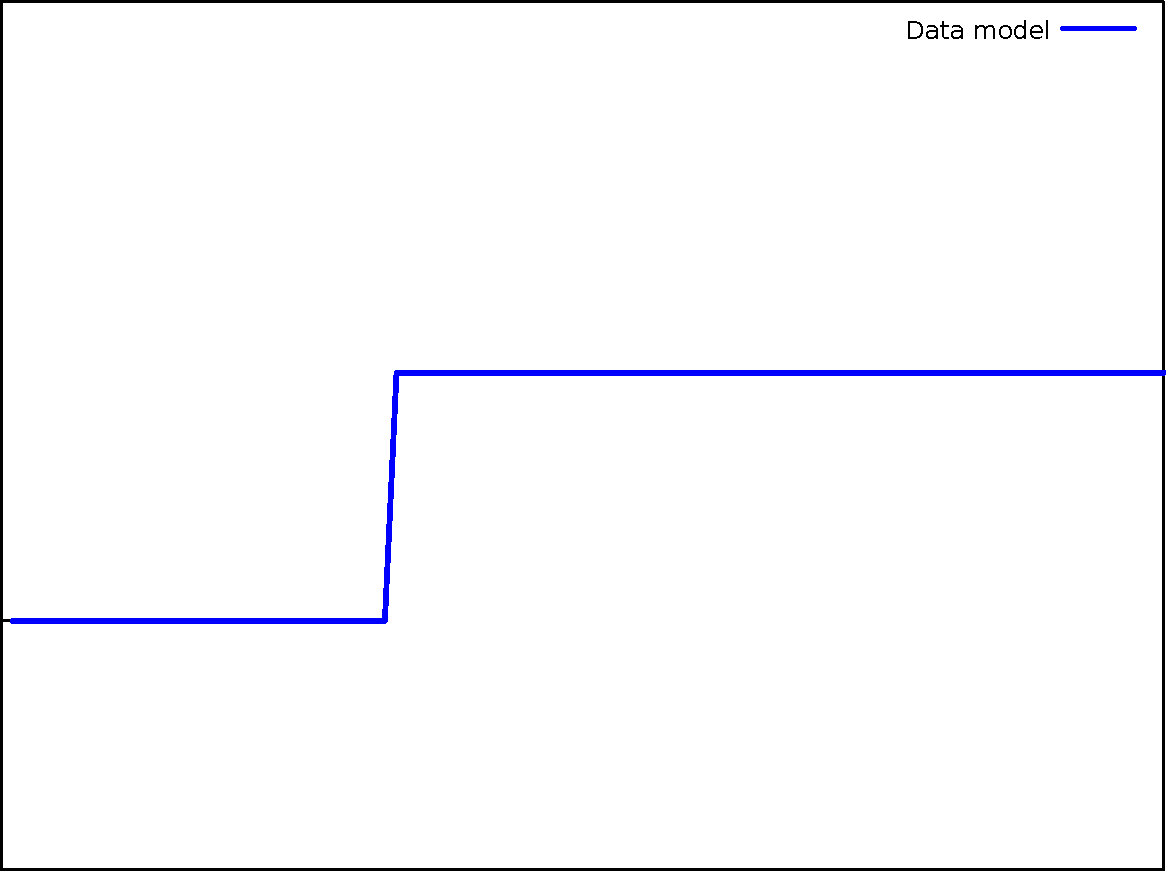
\includegraphics{images/data_bis.pdf}
      \end{axis}
      %% --------------------------------------------------------------------
          \end{tikzpicture}
          \caption*{Initial wavespeed model.}
          \label{1D_initial}
      \end{subfigure}
     \begin{subfigure}{0.45\textwidth}
        \centering
          \begin{tikzpicture}
      \begin{axis}[%
          width=\plotwidth, height=\plotheight,,
          at={(0,0)},scale only axis,separate axis lines,xminorticks=true,
          xlabel={\scriptsize{$x$}},
          %ylabel={$\velocity$},
          %%   ymode=log,
          yminorticks=true,
          ymin=900,ymax=1300
          %%   xmin=0.,xmax=100.
        ]

        %% load current data
        %% -----------------
        \addplot[color=blue!50!black,mark options={solid},
          forget plot,line width=1pt,
          mark size=2pt]
        table[x=monx,y=mony]
        {graph/VP100.dat};
      \end{axis}
      %% --------------------------------------------------------------------
          \end{tikzpicture}
          \caption*{Target wavespeed model.}
          \label{1D_target}
     \end{subfigure}
     \label{model_1D_target}
      \end{figure}
      }

\end{frame}


\begin{frame}{1D FWI problem}{Gradient validation}

  \setlength{\plotwidth}{6.0cm}
\setlength{\plotheight}{4.5cm}
   \begin{figure}
     \centering
         \begin{tikzpicture}
      \begin{axis}[%
          width=\plotwidth, height=\plotheight,,
          at={(0,0)},scale only axis,separate axis lines,xminorticks=true,
          xlabel={\scriptsize{$x$}},
          ylabel={\scriptsize{Gradient amplitude}},
          legend pos=south east
        ]
        %% load current data
        %% -----------------
        \addplot[color=black!50!black,mark options={solid}, mark = triangle,
          line width=1pt,
          mark size=0pt]
        table[x=monx,y=mony]
        {graph/grad_df.dat};
        \addlegendentry{\scriptsize{FD gradient}}

        \addplot[color=blue!50!black,mark options={solid}, mark = triangle,
          line width=1pt,
          mark size=0pt]
        table[x=monx,y=mony]
        {graph/grad_dto.dat};
        \addlegendentry{\scriptsize{DtO gradient}}


        \addplot[color=red!50!black,mark options={solid}, mark = triangle,
          line width=1pt,
          mark size=0pt]
        table[x=monx,y=mony]
        {graph/grad_otd.dat};
        \addlegendentry{\scriptsize{OtD gradient}}




        %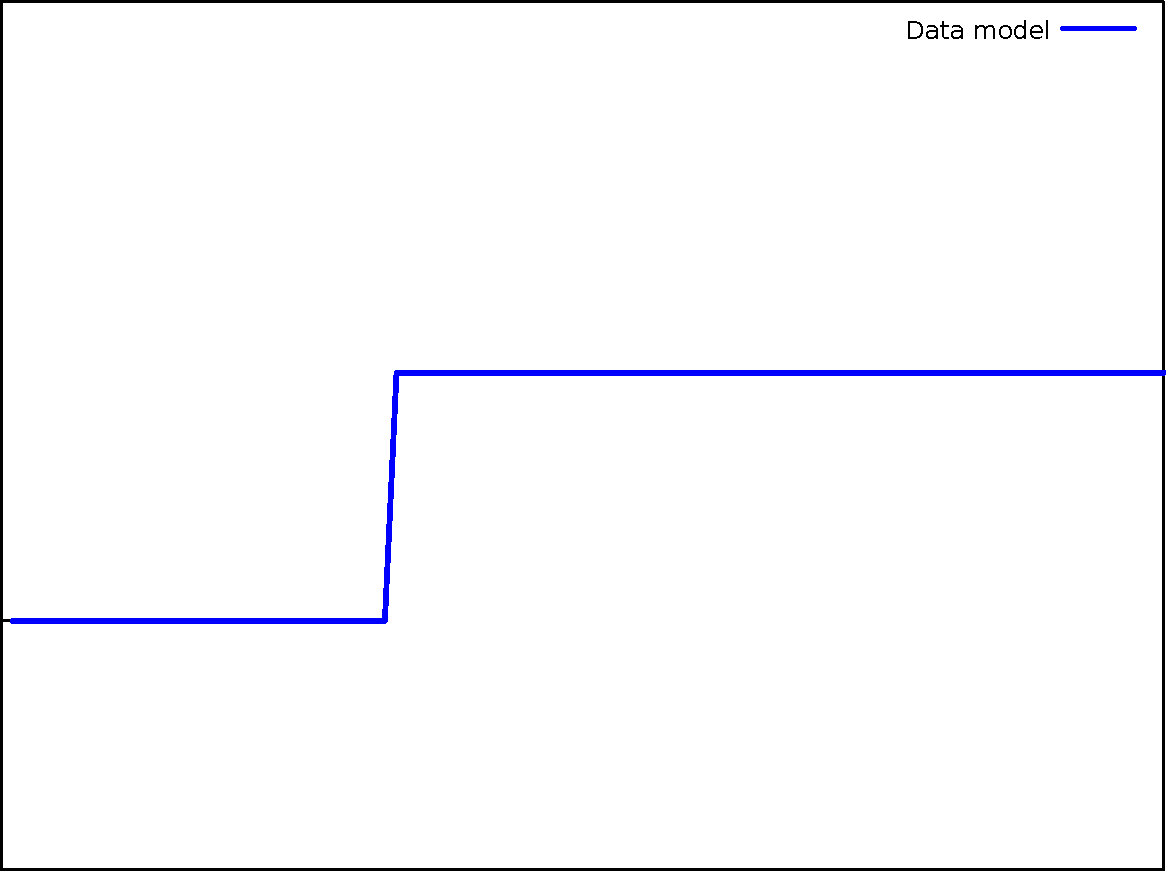
\includegraphics{images/data_bis.pdf}
      \end{axis}
      %% --------------------------------------------------------------------
         \end{tikzpicture}
     \end{figure}

\end{frame}


\begin{frame}{1D Results with L-BFGS}
        \pgfplotsset{every tick label/.append style={font=\tiny}}
      \setlength{\plotwidth} {4.5cm}
      \setlength{\plotheight}{3.0cm}
      \begin{figure}[!htbp]
        \begin{subfigure}{0.45\textwidth}
          \hspace{-0.5cm}
          \vspace{0.2cm}
        \centering
           \begin{tikzpicture}
      \begin{axis}[%
          width=\plotwidth, height=\plotheight,,
          at={(0,0)},scale only axis,separate axis lines,xminorticks=true,
          xlabel={\scriptsize{$x$}},
          ylabel={$\velocity$},
          %%   ymode=log,
          yminorticks=true,
          ymin=900,ymax=1300,
          legend pos=south east
          %%   xmin=0.,xmax=100.
        ]

        %% load current data
        %% -----------------
          \addplot[color=blue!50!black,mark options={solid}, mark = triangle,
          line width=1pt,
          mark size=1pt]
        table[x=monx,y=mony]
        {graph/vp_DTO.dat};
       \addlegendentry{DtO}

         \addplot[color=red!50!black,mark options={solid}, mark = *,
          line width=1pt,
          mark size=1pt]
        table[x=monx,y=mony]
        {graph/vp_OTD.dat};
        \addlegendentry{OtD}

      \end{axis}
      %% --------------------------------------------------------------------
          \end{tikzpicture}
           \caption*{\small{Final 1D wavespeed model reconstructed}.}
           \label{vp_DTO_vs_OTD}
      \end{subfigure}
      \begin{subfigure}{0.45\textwidth}
        \centering
          \begin{tikzpicture}
      \begin{axis}[%
          width=\plotwidth, height=\plotheight,,
          at={(0,0)},scale only axis,separate axis lines,xminorticks=true,
          xlabel={\scriptsize{iteration}},
          ylabel={$\CF$},
          ymode=log,
          yminorticks=true,
          %ymin=900,ymax=1300,
          legend pos=north east
          %%   xmin=0.,xmax=100.
        ]

        %% load current data
        %% -----------------
          \addplot[color=blue!50!black,mark options={solid}, mark = triangle,
          line width=1pt,
          mark size=1pt]
        table[x=monx,y=mony]
        {graph/run_lbfgs_DTO.dat};
       \addlegendentry{DtO}

         \addplot[color=red!50!black,mark options={solid}, mark = *,
          line width=1pt,
          mark size=1pt]
        table[x=monx,y=mony]
        {graph/run_lbfgs_OTD.dat};
        \addlegendentry{OtD}

      \end{axis}
      %% --------------------------------------------------------------------
          \end{tikzpicture}
          \caption*{\small{Cost function evolution through 400 L-BFGS iterations.}}
          \label{cf_DTO_vs_OTD}
         \end{subfigure}
         \end{figure}

\end{frame}


\begin{frame}
\begin{figure}
  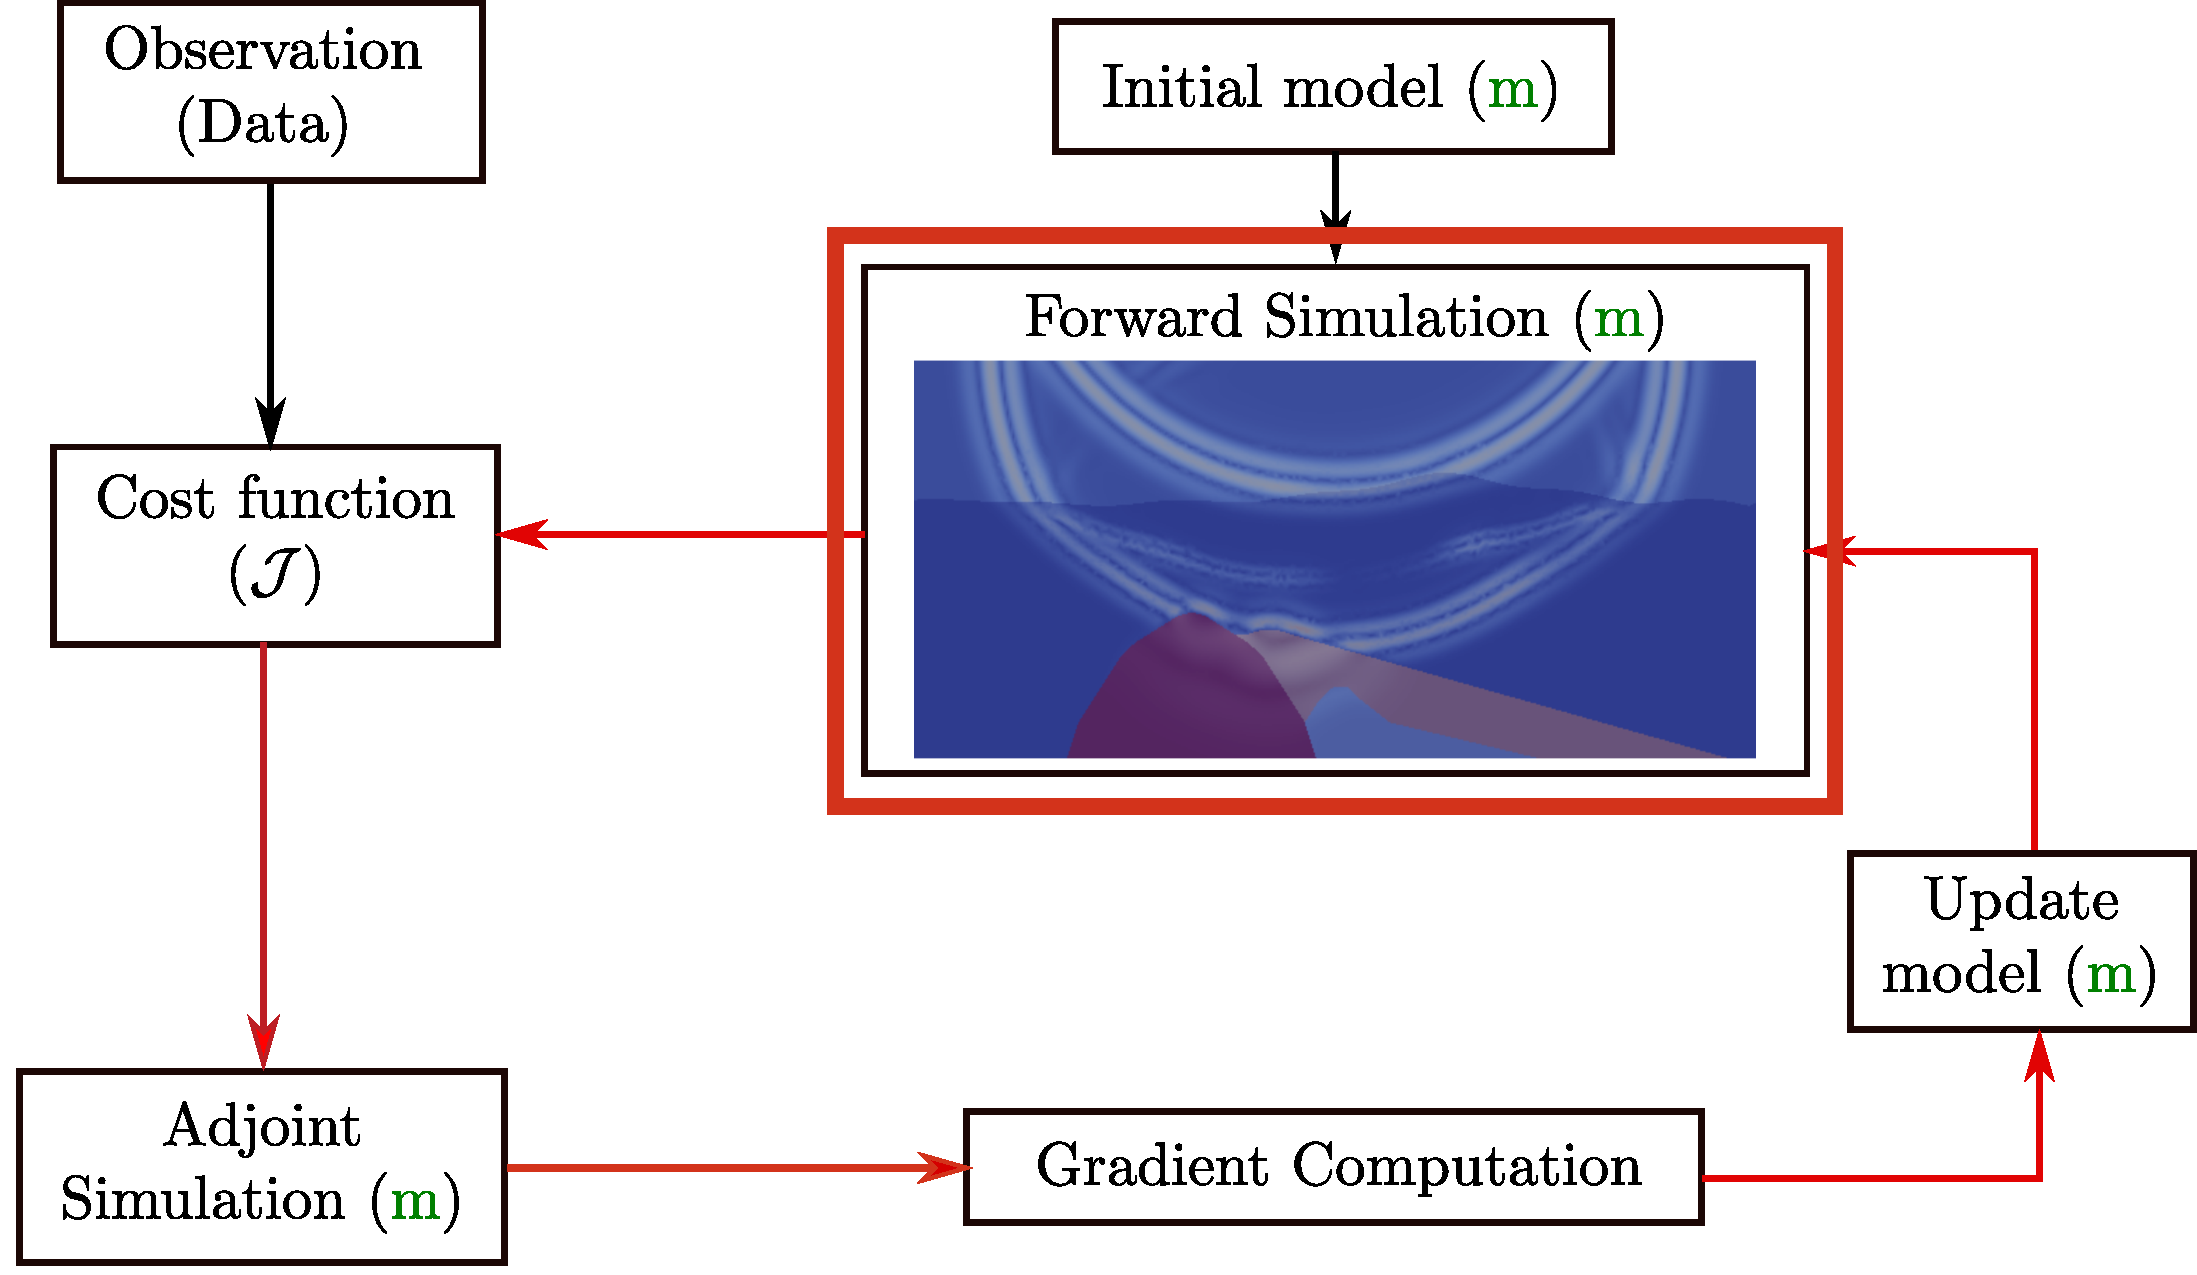
\includegraphics[scale=0.31]{image/fwi_workflow_red.pdf}
\end{figure}
\end{frame}

\begin{frame}[noframenumbering]
\begin{figure}
  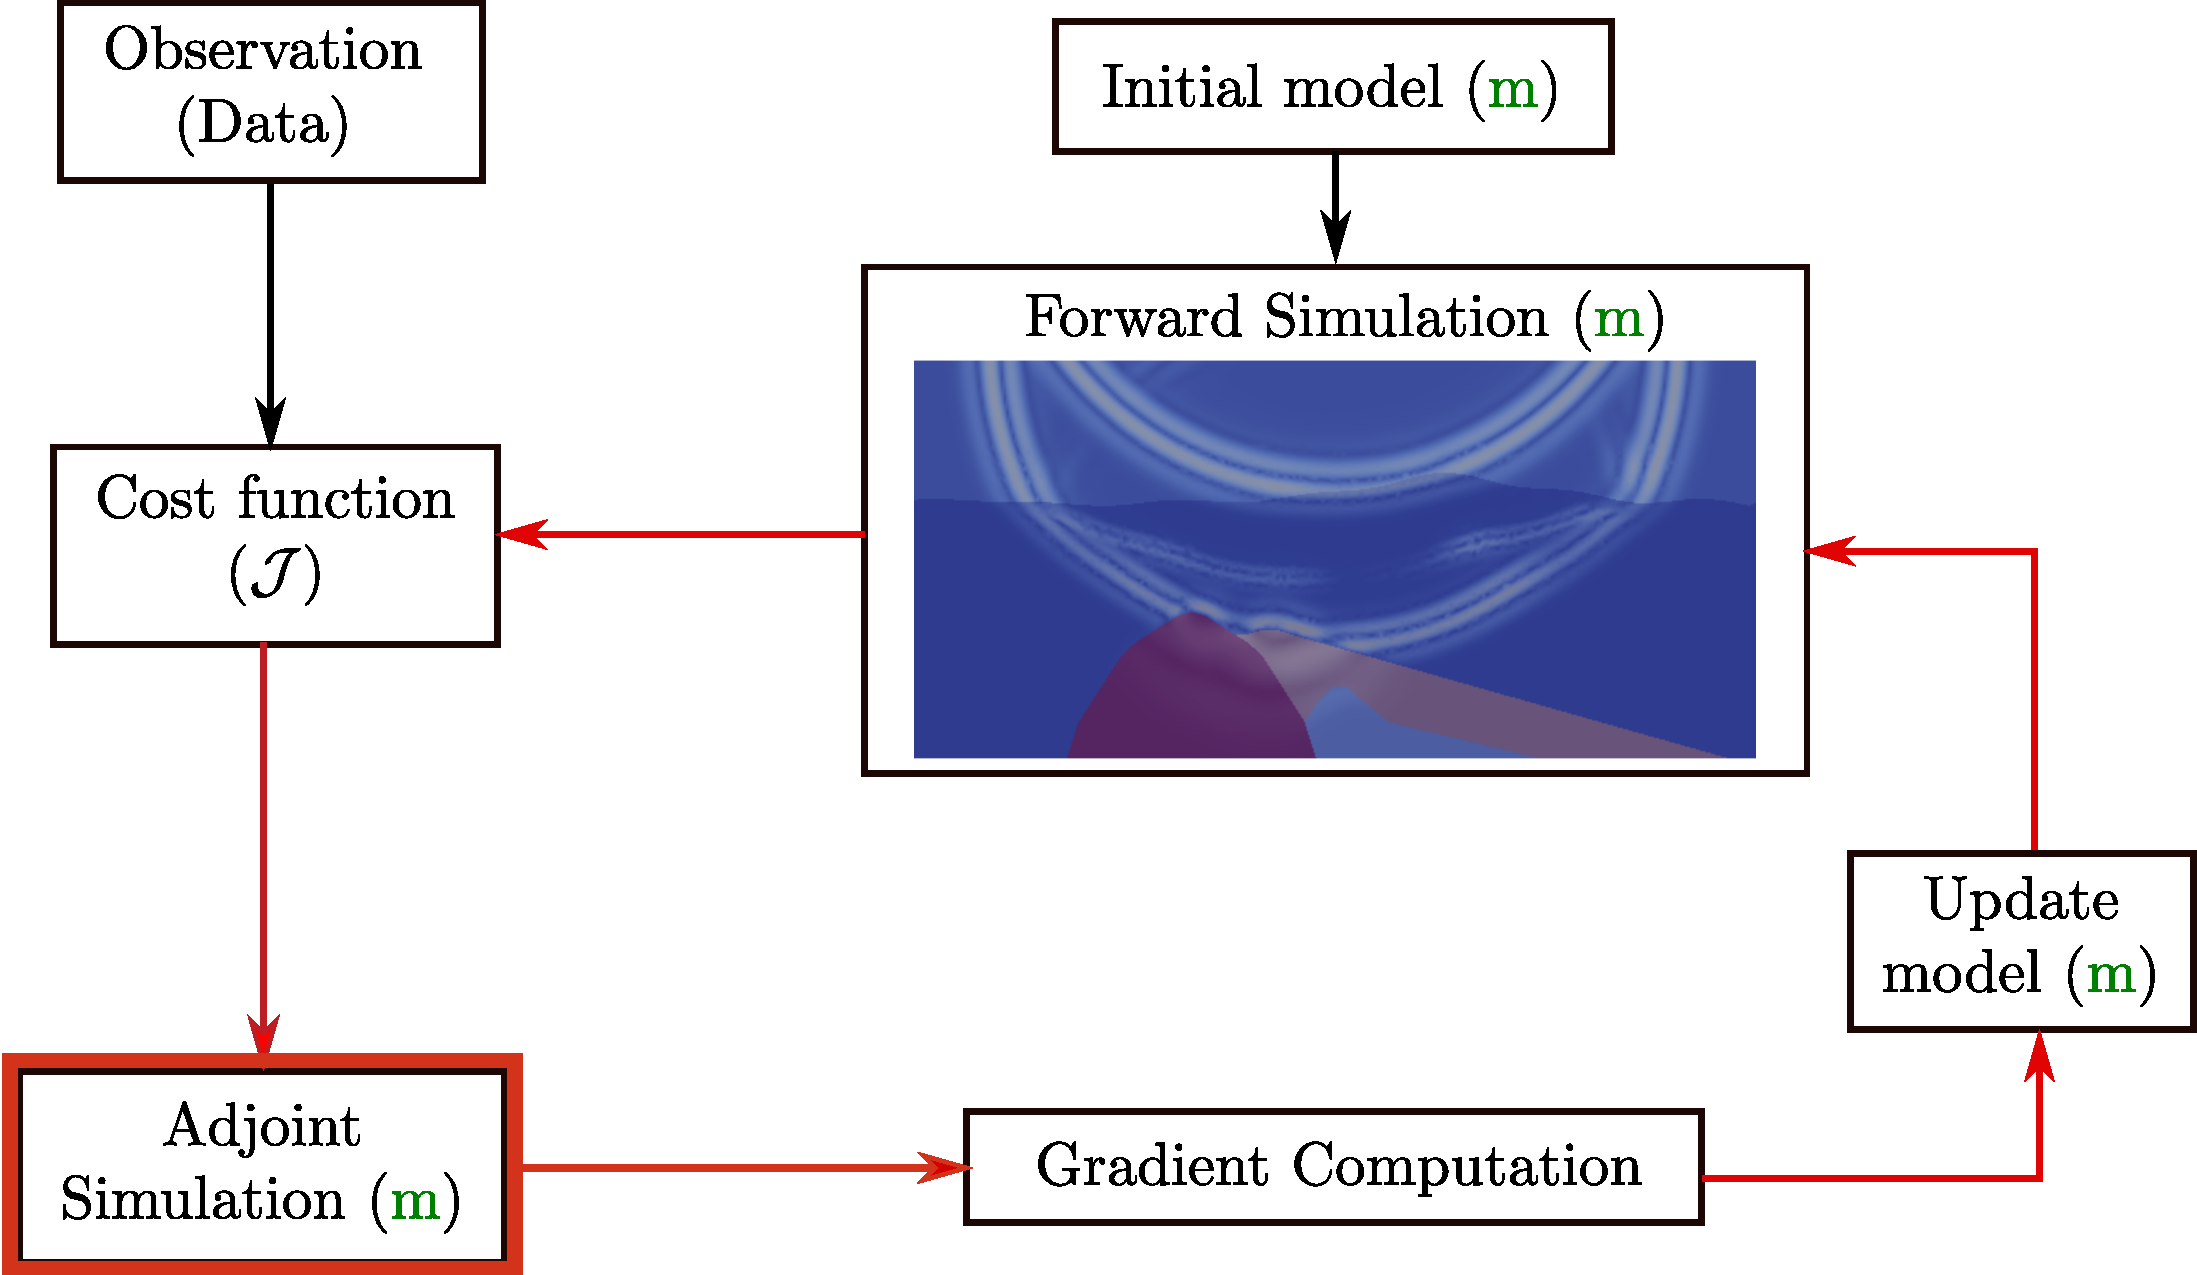
\includegraphics[scale=0.31]{image/fwi_workflow_red2.pdf}
\end{figure}
\end{frame}

\begin{frame}[noframenumbering]
\begin{figure}
  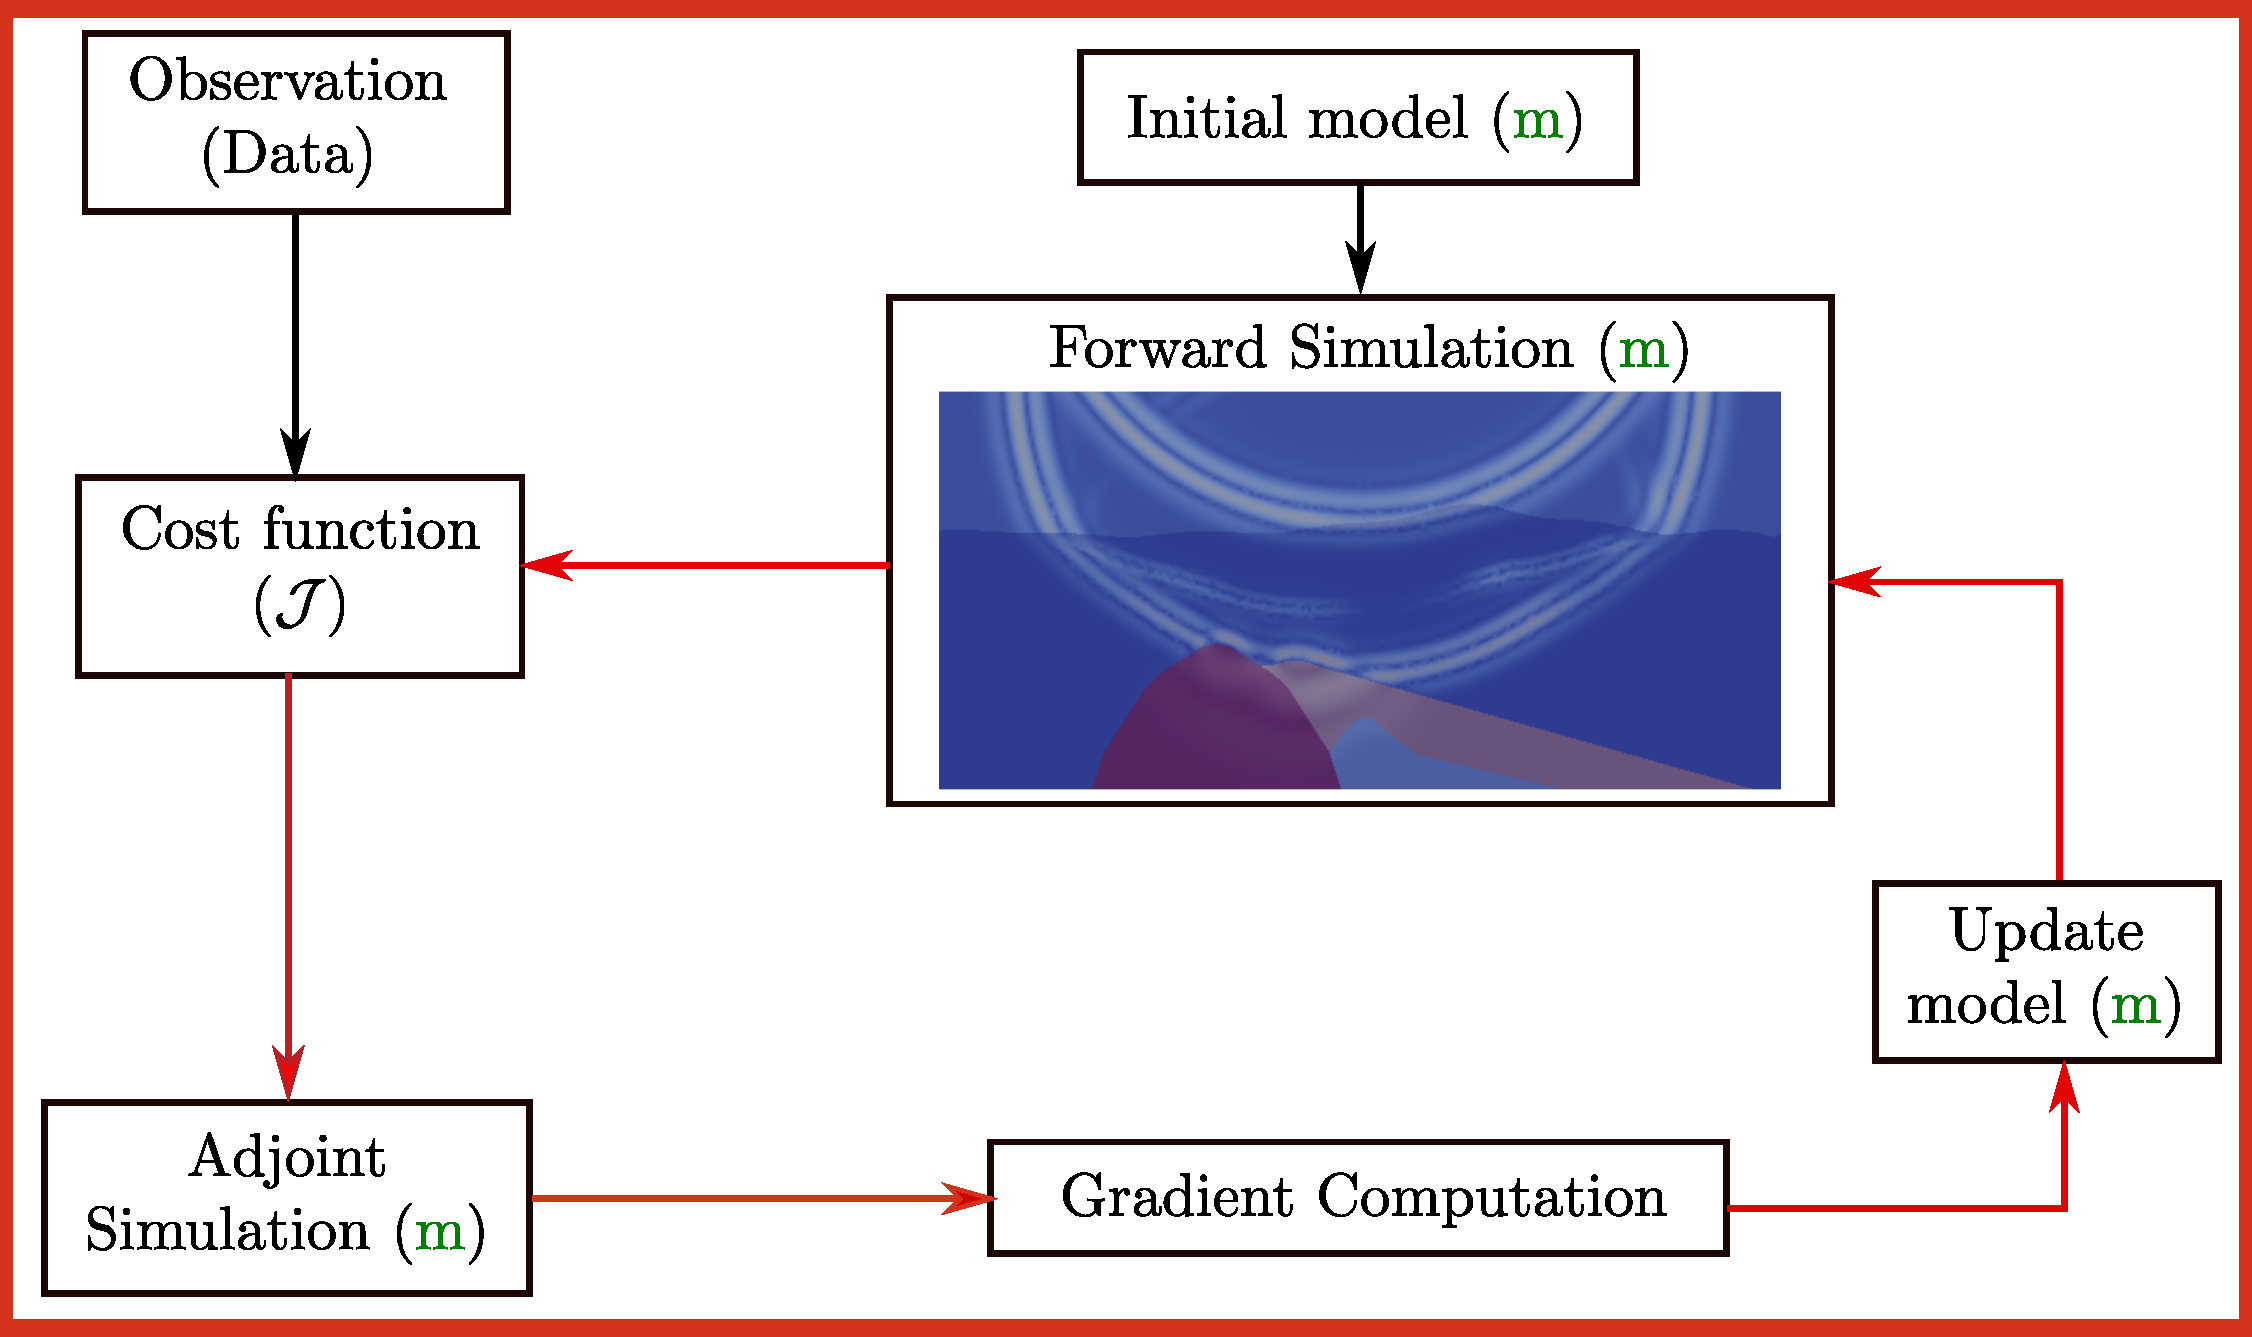
\includegraphics[scale=0.31]{image/fwi_workflow_all.pdf}
\end{figure}
\end{frame}








% ==========================================================
% ====== Frame : Choix et gradient expression ==============
% ==========================================================

%% \begin{frame}{Conclusion concerning the gradient expression}
%%   We chose the \textbf{Optimize then Discretize} strategy.


%%   \begin{overprint}
%%     \onslide<2>
%% \begin{block}{Gradient expression on the $l^{th}$ parameter for constant parametrization par element ($\frac{1}{\bm}{\density}$).}
%%   \begin{align}
%% (\frac{\partial}{\partial \frac{1}{\bm}_l} \CF(\smodel))_h  &\approx \deltat \detJKl \sum_{n=0}^\nt  (\frac{\partial}{\partial t} {{\boldsymbol{\textcolor{\myred}{\scoefPolP}}^n)}^{\element^l}}^\top \MassRef  {(\boldsymbol{\textcolor{\myred}{\scoefAdjP}}^n)}^{\element^l}\,,
%% \end{align}
%% and
%% \begin{align}
%% (\frac{\partial}{\partial \density_l} \CF(\smodel))_h  &\approx \deltat \detJKl \sum_{d=1}^\dim \sum_{n=0}^\nt  (\frac{\partial}{\partial t} {{\boldsymbol{\textcolor{\myred}{\scoefPolVd}}^n)}^{\element^l}}^\top \MassRef  {(\boldsymbol{\textcolor{\myred}{\scoefAdjVd}}^n)}^{\element^l} \,.
%% \end{align}
%% \end{block}

%% \onslide<3>
%% \vspace{-0.3cm}
%% \begin{block}{Gradient expression for \textbf{WADG} parametrization for the the $q^{th}$ quadrature point on the $l^{th}$ element ($\frac{1}{\bm}{\density}$).}
%%   \begin{align}
%% \left(\frac{\partial}{\partial \frac{1}{\bm}_{l,q}} \CF(\smodel)\right)_h \approx  \deltat \detJKl \sum_{n=0}^\nt  {{\textcolor{\myred}{\coefPolP}^n}^{\element^l}}^\top \Pquad  diag(\weight \boldsymbol{\delta_q}) \Pquad^\top   {\textcolor{\myred}{\coefAdjP}^n}^{\element^l} \,,
%% \end{align}
%% and
%% \begin{align}
%% \left(\frac{\partial}{\partial \density_{l,q}} \CF(\smodel)\right)_h \approx \deltat \detJKl \sum_{n=0}^\nt \sum_{d=1}^\dim {{\textcolor{\myred}{\coefPolV}^n}^{\element^l}}^\top \Pquad diag(\weight \boldsymbol{\delta_q}) \Pquad^\top   \boldsymbol{\textcolor{\myred}{\scoefAdjVd}}^{\element^l} \,.
%% \end{align}
%% \end{block}
%% \end{overprint}

%%   \end{frame}
